%!TEX root = ../thesis_a4.tex
% Some new commands for setting up appendices
\newcommand\contrib[1]{\\~{\footnotesize (#1)}}
% 
\newcommand\resource[2]{
	\noindent #1 \par
	\vspace{0.2em}
	{\centering	\url{#2} \par}
	\vspace{0.5em}
	\hrule \par 
	\vspace{0.8em} \par}
%
%
\chapter[Publications by the Author][Publications by the Author]{Publications by the Author}
\label{app:mypapers}% by the author

%We here provide a list of publications by the author related with the thesis work. For the publications where the role is not that of the first author we also specify the contributions. Wherever not specified, the contributions are mainly in the formulation of the research problem, building the dataset, writing the code, performing the experiments, analyzing the results and writing the manuscript.

\subsection*{Peer-reviewed journals}
\begin{itemize}[leftmargin=*]
	\item \textbf{Ó Nuanáin, C.}, Herrera, P., \& Jordà, S. (2017). Rhythmic Concatenative Synthesis for Electronic Music: Techniques, Implementation, and Evaluation. \textit{Computer Music Journal}, 41(2), pp. 21–37.
%	\contrib{Companion webpage: \url{http://compmusic.upf.edu/node/323}}
	\item Vogl, R., Leimeister, M., \textbf{Ó Nuanáin, C.}, Jord, S., Hlatky, M., \& Knees, P. (2016). An Intelligent Interface for Drum Pattern Variation and Comparative Evaluation of Algorithms. \textit{Journal of the Audio Engineering Society}, 64(7), pp. 503–513.
%	\contrib{Formulating methodology, Writing parts of the code}
	
\end{itemize}
%
\subsection*{Full articles in peer-reviewed conferences}
\begin{itemize}[leftmargin=*]
	\item \textbf{Ó Nuanáin, C.}, Jordà, S., \& Herrera, P. (2017). k -Best Hidden Markov Model Decoding for Unit Selection in Concatenative Sound Synthesis. In \textit{Proceedings of the International Symposium on Computer Music Multidisciplinary Research (CMMR)}. Porto, Portugal.
	\item \textbf{Ó Nuanáin, C.}, Herrera, P., \& Jordà, S. (2016). An Evaluation Framework and Case Study for Rhythmic Concatenative Synthesis. In Proceedings of the International Society for Music Information Retrieval Conference (ISMIR). New York, USA.
	\item \textbf{Ó Nuanáin, C.}, Jordà, S., \& Herrera, P. (2016). An Interactive Software Instrument for Real-time Rhythmic Concatenative Synthesis. In Proceedings of the International Conference on New Interfaces for Musical Expression (NIME). Brisbane, Australia.
	\item \textbf{Ó Nuanáin, C.}, Jordà, S., \& Herrera, P. (2016). Towards User-Tailored Creative Applications of Concatenative Synthesis in Electronic Dance Music. In \textit{Proceedings of the International Workshop on Musical Metacreation (MUME)}. Paris, France.
	\item \textbf{Ó Nuanáin, C.}, Herrera, P., \& Jordà, S. (2015). Target-Based Rhythmic Pattern Generation and Variation with Genetic Algorithms. In \textit{Proceedings of the Sound and Music Computing Conference (SMC)}. Maynooth, Ireland.
	\item \textbf{Ó Nuanáin, C.}, \& Sullivan, L. O. (2014). Real-time Algorithmic Composition with a Tabletop Musical Interface - A First Prototype and Performance. In \textit{Proceedings of Audio Mostly: A Conference on Interaction With Sound}. Aalborg, Denmark.
	%	
\end{itemize}
%
\subsection*{Other contributions to conferences}
\begin{itemize}[leftmargin=*]
	\item Faraldo, Á., \textbf{Ó Nuanáin, C.}, Gómez, D., Herrera, P., \& Jordà, S. (2015). Making Electronic Music with Expert Musical Agents. In \textit{Late-Breaking Demo Session of the International Society for Music Information Retrieval Conference (ISMIR)}. Málaga, Spain.
	\item \textbf{Ó Nuanáin, C.}, Hermant, M., Faraldo, Á., \& Gómez, D. (2015). The EEEAR: Building a Real-Time MIR-Based Instrument from a Hack. In \textit{Late-Breaking Demo Session of the International Society for Music Information Retrieval Conference (ISMIR)}. Málaga, Spain.
\end{itemize}



%%%%%%%%%%%%%%%%%%%%%%%%%%%%%%%%%%%%%%%%%%%%%%%%%%%%%%%%%%%%%%%%%%%%%%%%%%%%%%
%%%%%%%%%%%%%%%%%%%%%%%%%%%%%%%%%%%%%%%%%%%%%%%%%%%%%%%%%%%%%%%%%%%%%%%%%%%%%%

\chapter{Listening Survey Web Tool}\label{app:listening_survey}

Over the course of this doctoral thesis a need arose for a flexible system that could perform comparative listening surveys and evaluation with ease. As a consequence, a web platform was developed that is easy to setup, customise, configure and deploy etc. The main advantage of this is that surveys can be conducted remotely by the user without the requirement of supervision and physical presence. The tool and its source code is freely available online \footnote{\url{https://github.com/carthach/listener_survey_tool}}, and has since been used in other researchers' works \citep{Marti2015, Jade2016}.

An initial landing page (\figref{fig:survey_landing}) provides instructions for the participants along with an estimation of the time and the number of questions. The participant then fills out personal details that are gathered anonymously - no names or contact details are recorded - followed by some descriptive questions pertinent to the survey being conducted. For instance, in the case of our rhythm surveys we were interested to know the musical training of each participant and whether that was concentrated in more percussive practice.  

The questionnaire commences (\figref{fig:survey_page}) with a series of randomised questions consisting of a target sound to be listened to and several other generated sounds that necessitate scrutiny. Repeated listening is possible before making a final decision on the Likert score for each question.

To make the tool as easy as possible to deploy, database dependency is avoided. Subsequent to each participant's concluded survey session, a CSV file of the completed questionnaire results are simply mailed to the researcher's email address.


\begin{sidewaysfigure}
	\begin{center}
		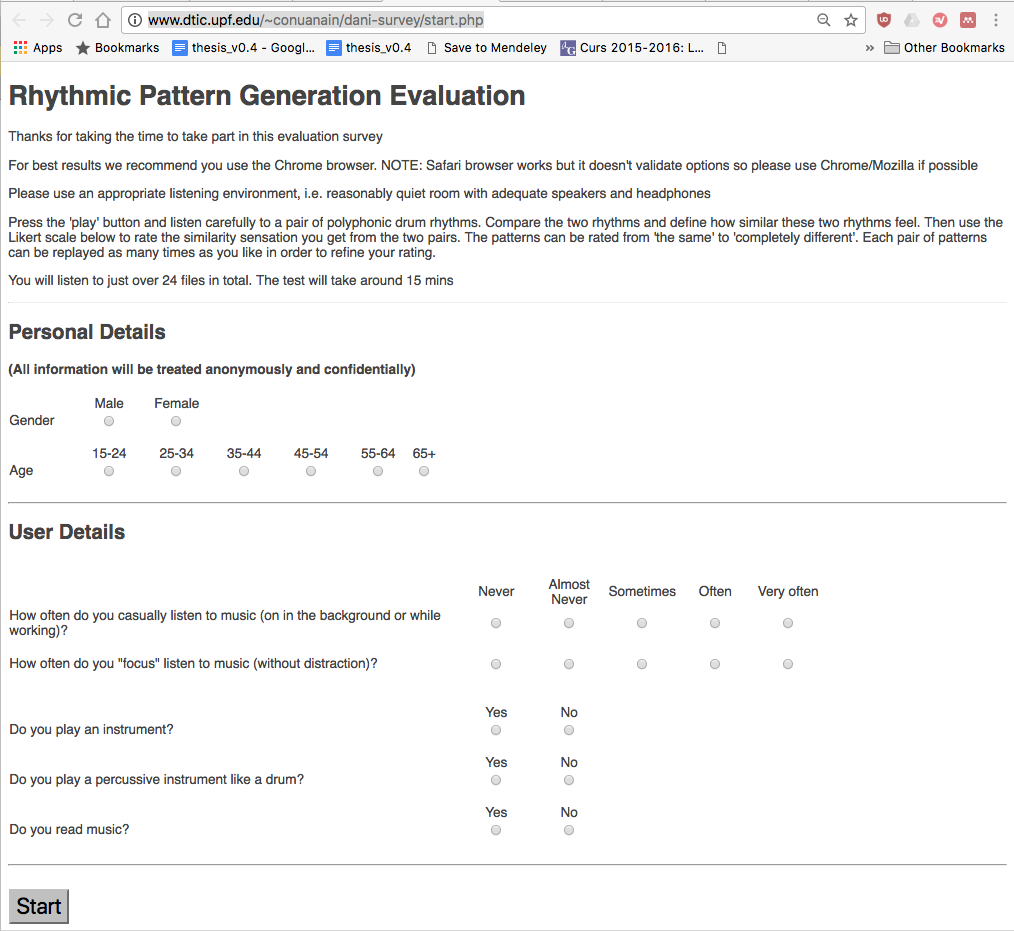
\includegraphics[width=0.75\textwidth]{ch99/figures/survey_landing.png}
	\end{center}
	\caption[Web Survey Landing Page]{Web Survey Landing Page}
	\label{fig:survey_landing}
\end{sidewaysfigure}

\begin{sidewaysfigure}
	\begin{center}
		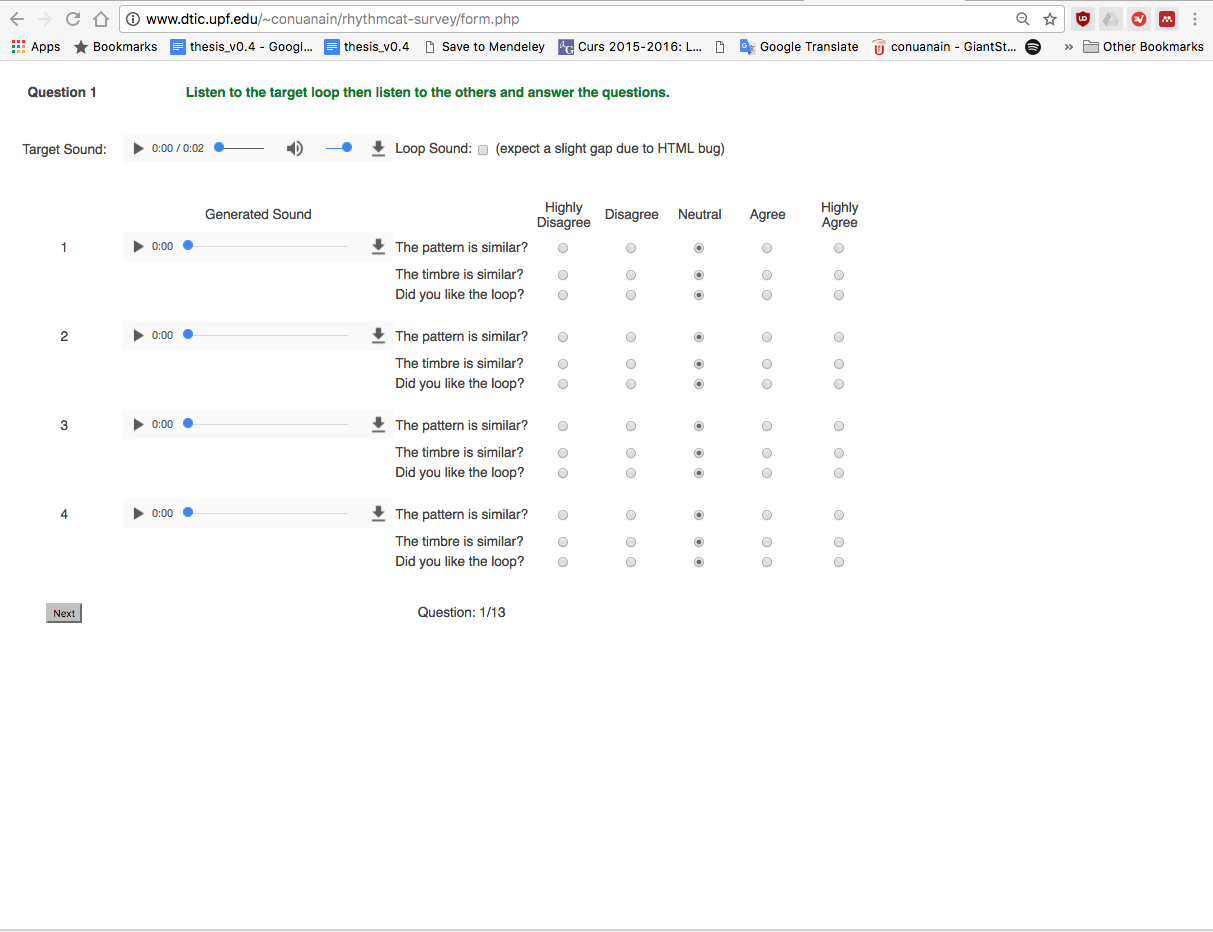
\includegraphics[width=0.75\textwidth]{ch99/figures/survey_page.png}
	\end{center}
	\caption[Web Survey Question Page]{Web Survey Question Page}
	\label{fig:survey_page}
\end{sidewaysfigure}

\chapter{Resources}\label{app:resources}

%In this appendix, we provide the URLs to access the resources related to this thesis, which include the code and tools, the corpora and test datasets, and the applications and demos. An up-to-date links of all these resources is maintained on the companion web page of this thesis: \url{http://compmusic.upf.edu/node/304} (mirrored at \url{http://www.sankalpgulati.in/phd-thesis.html}).

\section*{Code and Tools}

\subsection*{Implementation of Methods}
Implementation of the methods presented in this thesis are made publicly available for research purposes. We also indicate (in squared brackets) the language in which the implementation is available. Other frameworks and libraries are also listed.

\begin{itemize}
	\item SimpleGA [C++]
	\item RhythmGA [C++]
	\item GenDrum [Max/MSP and Max for Live]
	\item kViterbi [Python] 
	\item PyConcat [Python]
	\item RhythmCAT [C++ (JUCE)]
\end{itemize}

\subsection*{Tools}

\begin{itemize}
	\item Essentia audio analysis library (\url{http://essentia.upf.edu/})
	\item Librosa audio analysis library (\url{https://github.com/librosa/librosa})
	\item Madmom audio analysis library (\url{https://github.com/CPJKU/madmom})
	\item Scikit-learn machine learning library (\url{http://scikit-learn.org/stable/})
	\item OpenCV computer vision library (\url{https://opencv.org/})
	\item Boost Graph Library (\url{http://boost.org/})
	\item JUCE cross platform C++ framework (\url{http://juce.com/})
\end{itemize}


\section*{Corpora and Datasets}

Corpora and datasets used throughout the thesis are summarised here and are categorised by those contributed by the authors as well as those that were made available by other researchers.

\subsection*{Author Contributed}

\begin{itemize}
	\item `Orchestral Timbre' collection used in the classification experiment (\secref{sec:corpus_carnatic_music_corpus}) \\ 
	Sound files, extracted features, classifier models and IPython notebooks can be downloaded here:\\
	\url{http://github.com/carthach/phd_thesis/tree/master/classification/drums/data}
	\item `Drum Timbre' collection used in the classification experiment (\secref{sec:corpus_carnatic_music_corpus}) \\ 
	Sound files, extracted features, classifier models and IPython notebooks can be downloaded here:\\
	\url{github.com/carthach/phd_thesis/tree/master/classification/orchestra/data}	
	\item `Breakbeat' collection used in the evaluation of RhythmCAT(\secref{sec:corpus_carnatic_music_corpus}) \\ 
	Sound files and annotations can be downloaded here:\\
	\url{http://www.github.com/carthach/thesis/experiments/evaluation/data}	
%	\item `Dunya Carnatic CC' and `Dunya Hindustani CC' collection in MusicBrainz forms the open-access music corpus (\secref{sec:corpus_open_access_research_corpus}) \\
%	\url{https://musicbrainz.org/collection/a163c8f2-b75f-4655-86be-1504ea2944c2}\\
%	\url{https://musicbrainz.org/collection/6adc54c6-6605-4e57-8230-b85f1de5be2b}
\end{itemize}

\subsection*{Public Datasets}

\begin{itemize}
  \item ENST-Drums: Provided by Télécom ParisTech \citep{Gillet2006}, contains an audio-visual annotated dataset of performances by 3 professional drummers using multi-track studio recording in a variety of configurations (single hits, phrases and accompaniments) and a variety of styles including jazz and rock. \\
Summary and ordering details are available here:\\
	\url{http://perso.telecom-paristech.fr/~grichard/ENST-drums/}
  \item Modal (Musical Onset Dataset And Library): Hand annotated, contains 501 onsets across 71 files containing a mix of mostly monophonic events \citep{Glover2011}\\
Datset can be downloaded from:\\
\url{https://github.com/johnglover/modal}
  \item JKU: Contains 321 files with 27,774 total onsets. Compiled from a number of different sources by Sebastian Böck for evaluating his SuperFlux algorithm \citep{Bock2013}. The algorithm was developed especially to handle vibrato, and accordingly the dataset contains a large number of samples that purposely addressing vibrato, such as samples from opera or classical technique strings.\\
Annotations and some audio can be downloaded from here:\\
\url{https://github.com/CPJKU/onset_db}
\end{itemize}
%
%The corpora and the test datasets compiled in the CompMusic project for all the music traditions are available at:
%\begin{description}[style=nextline]
%	\item[CompMusic music corpora] \url{http://compmusic.upf.edu/corpora}
%	\item[CompMusic test datasets] \url{http://compmusic.upf.edu/datasets}
%\end{description}
%
%
%\section*{Applications and Demos}
%
%\begin{itemize}
%	\item Discovered melodic patterns:
%	\begin{itemize}
%		\item Metadata-wise browsing: \url{dunya.compmusic.upf.edu/motifdiscovery}
%		\item Network of melodic patterns: \url{dunya.compmusic.upf.edu/pattern_network/}
%		\item We also share the database of the discovered melodic patterns that contains the time-stamps, similarity with the other patterns, and the corresponding recording information for all the patterns.
%	\end{itemize}
%	\item \gls{ragawise}:
%	\begin{itemize}
%		\item Web interface: \url{https://dunya.compmusic.upf.edu/ragawise/}
%		\item Code: \url{https://github.com/sankalpg/ragawise}
%	\end{itemize}
%	
%	\item Mobile applications:
%	\begin{itemize}
%		\item \Gls{saraga}: \url{https://play.google.com/store/apps/details?id=com.musicmuni.saraga}
%		\item \Gls{riyaz}: \url{https://play.google.com/store/apps/details?id=com.musicmuni.riyaz}
%	\end{itemize}
%\end{itemize}
%
%We reiterate that the links provided for some of these resources may change over time. An up-to-date links of all these resources are maintained on the companion web page of this thesis: \url{http://compmusic.upf.edu/node/304} (mirrored at \url{http://www.sankalpgulati.in/phd-thesis.html}).

\chapter{The PyConcat Library}
\label{app:pyconcat}

\section{Description}

The PyConcat \footnote{Not to be confused with \url{https://github.com/thomasballinger/pyconcat} a script for concatenating Python sripts. I really need to come up with more original name for my software.} library is a Python environment for conducting research-oriented concatenative synthesis of signals. It uses feature extraction routines from Essentia and Librosa as well as distance measures from scipy and novel unit selection via \textit{k}-Best Viterbi.

The basic pipeline for performing concatenative synthesis with this tool is as follows.

\begin{enumerate}
  \item \textbf{Segmentation}
\begin{itemize}
  \item Framewise in the time domain or using \acrshort{fft}/\acrshort{ifft} resynthesis 
  \item Onsts
  \item Beats
\end{itemize}
\item \textbf{Feature Analysis}
\begin{itemize}
\item Temporal: loudness, attack
\item Spectral: flatness, centroid
\item Timbral: \acrshort{bfcc}s, \acrshort{mfcc}s, \acrshort{gfcc}s
\item Musical: f0, \acrshort{hpcp}s
\end{itemize}
\item \textbf{Unit Selection}
\begin{itemize}
  \item Linear Search
  \item \textit{k}-D Tree
  \item Viterbi
  \item \textit{k}-Best Viterbi
\end{itemize}
\end{enumerate}

\section{API}

A concatenative synthesis task is performed in stages in accordance with the previous pipeline. Separate statements segment the units and compute features before finally combining a sequence with unit selection. This also allows the flexible separation of unit scale segmentation and features that allow different specifications for target and corpus unit. 

The code snippet below shows an example of extracting units from the target at the beat unit scale while concatenating the top 10 sequences at the onset scale using Viterbi decoding and time-stretching.

\small
\begin{lstlisting}[language=Python]

e = Extractor.Extractor()

#Find all the corpus files in the path
corpusFiles = extractor.getListOfWavFiles(corpusPath)

#Extract features and units
tFeatures, tUnits, tUnitTimes = e.analyseFile(targetFile, 
						scale="beat")
						
cFeatures, cUnits, cUnitTimes = e.analyseFiles(corpusFiles, 
						writeOnsets=True, 
						scale="onsets")

#Get list of candidate sequences with k-Best Viterbi Decoding 
sequences = unitSelection.unitSelection(tFeatures, 
					cFeatures, 
					method="kViterbiParallel", 
					normalise="MinMax", 
					topK=10)

# Concatenate the sequences with time stretching
audio = e.concatOnsets(sequences, 
			corpusUnits, 
			targetUnits, 
			stretchUnits=True)	
							   
e.writeAudio(audio, "out.wav")
 
\end{lstlisting}

\normalsize

\section{Links}

\begin{itemize}
  \item Documentation - \url{http://pyconcat.readthedocs.io/en/latest/source/PyConcat.html}
  \item Library - \url{https://github.com/carthach/pyconcat}
\end{itemize}

\chapter{Related Applications}
\label{app:related_applications}

\section{The Eear - Enhanced DJ Assistant}

The Eear\footnote{\url{http://carthach.github.io/eear/}} was prototyped by members of The GiantSteps team over a 24-hour period at the Sónar Music Hack Day in 2014 and subsequently won the MusicBricks category for best hack. A more refined version of the system was developed for mobile and desktop and selected for presentation at the Music Tech Fest in Slovenia, as well as the late breaking demo session at ISMIR 2015, in Málaga \citep{ONuanain2015}. A lot of the feature extraction and segmentation logic that was described in this thesis was also used to develop this system.

The Eear comprises a mobile application (\figref{fig:eear} - left) that uses the microphone of the device to capture live input from any source and perform harmonic analysis (using a rolling average of the \acrshort{hpcp} vector) in order to estimate the current chord or key. This key and scale information is sent via \acrshort{osc} to a \acrshort{vst} plugin (\figref{fig:eear} - right) that allows \acrshort{mpc} style sampling of related sounds filtered by that very same tonal information - thus it selects units that are always `in key' with the live input captured by the mobile.

\section{Atomix}

For the 2017 edition of the Sónar Innovation Challenge\footnote{\url{http://sic.upf.edu/challenges/}}, members of the \acrshort{mtg} team proposed and mentored a project that challenged selected participants to prototype a system that somehow combined the spirit of timbre space driven concatenative synthesis with state of the art source separation technology.

While the team eventually devised their own tools and did not implement any source separation, the concept art by Olivia Andrieux (\figref{fig:atomix}) shows how it could be realised visually with RhythmCAT-inspired visualisation and interaction for each track of stream of audio.

\begin{figure}
	\begin{center}
		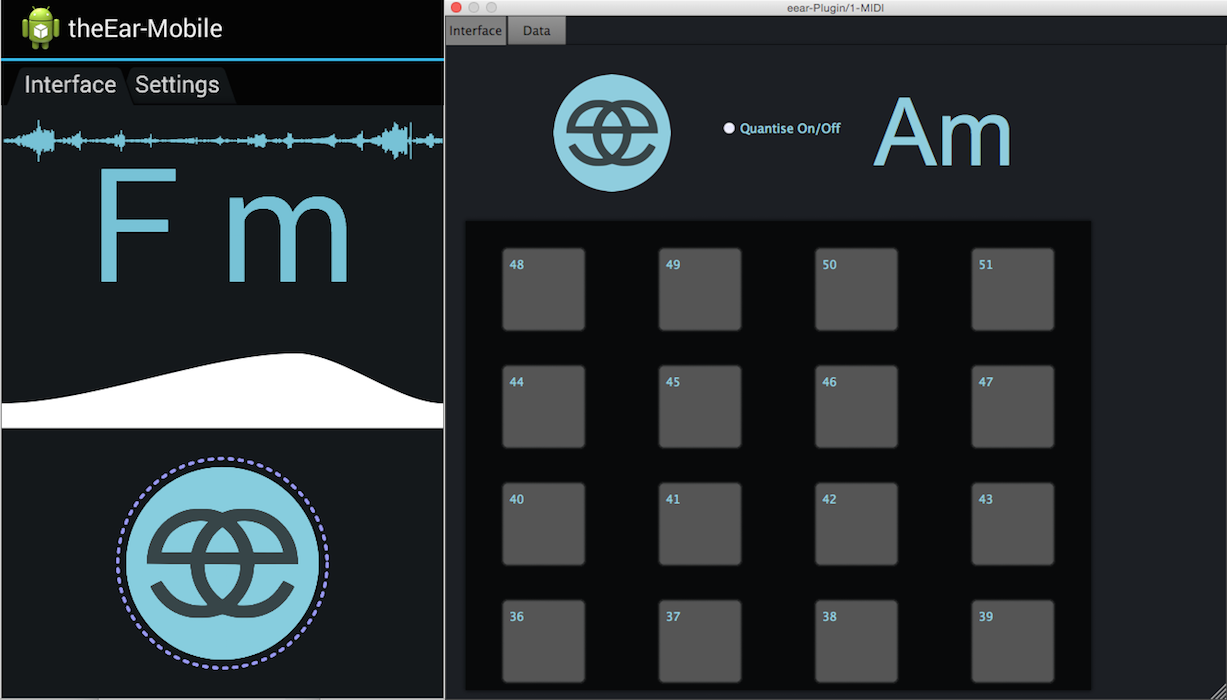
\includegraphics[width=0.9\textwidth]{ch99/figures/combined.png}
	\end{center}
	\caption[The Snitch Enhanced DJ Assistant Mobile and Plugin Interface]{The Snitch, mobile app (left), plugin interface (right)}
	\label{fig:eear}
\end{figure}

\begin{figure}
	\begin{center}
		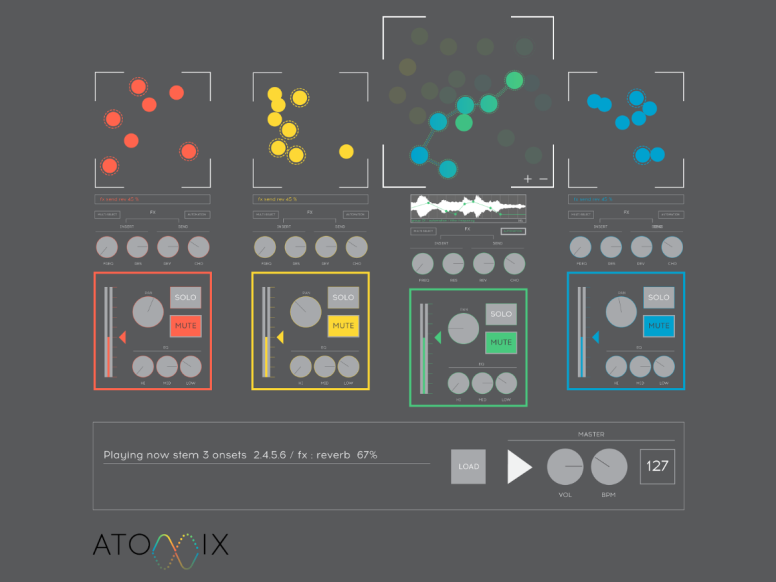
\includegraphics[width=0.9\textwidth]{ch99/figures/atomix.png}
	\end{center}
	\caption[Atomix User Interface]{Atomix User Interface. Image from Centre for Digital Music at Queen Mary.}
	\label{fig:atomix}
\end{figure}

%%%%%%%%%%%%%%%%%%%%%% Another appendix!  %%%%%%%%%%%%%%%%%%%

%\chapter{Additional Figures and Tables}
%\label{app:additional_material}

	
%\begin{figure}[h]
%	\begin{subfigure}{\textwidth}
%		\centering
%		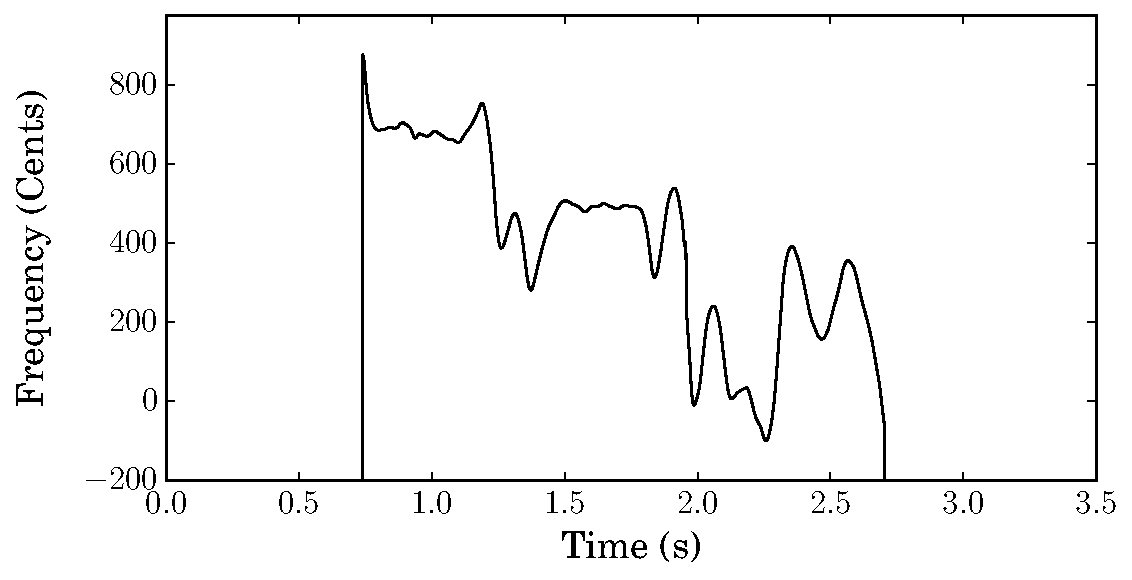
\includegraphics[width=\figSizeSeventy]{ch01_introduction/figures/Sphuritam_on_M1_Raga_Arabhi.pdf}
%		\caption{\Gls{sphuritam} \gls{gamaka}\protect\footnotemark}
%		\label{fig:sphuritam_todi}
%	\end{subfigure}
%	\begin{subfigure}{\textwidth}
%		\centering		
%		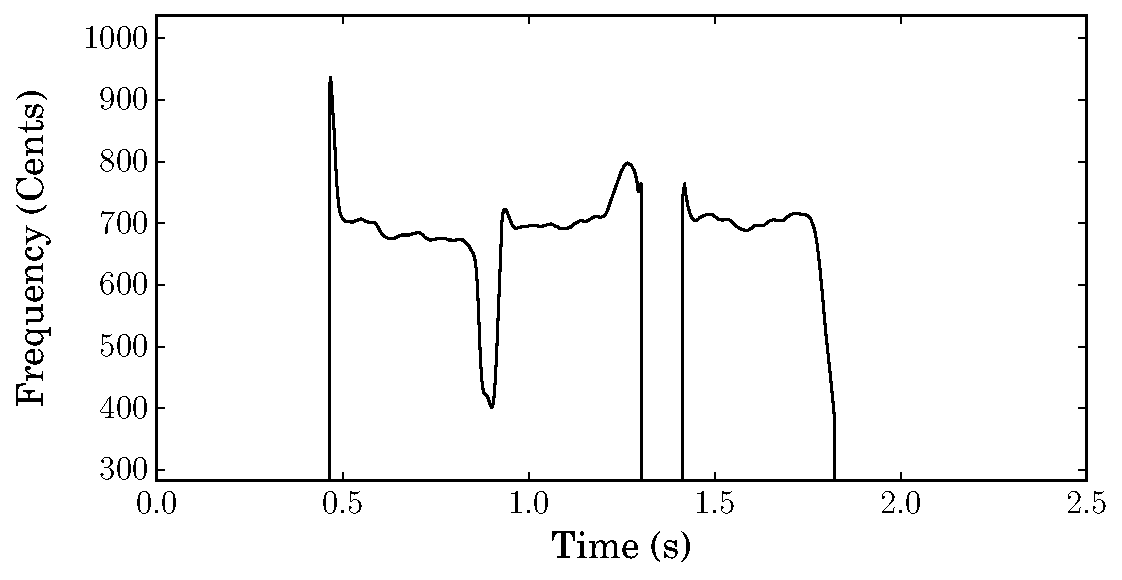
\includegraphics[width=\figSizeSeventy]{ch01_introduction/figures/Odukkal_on_D1.pdf}
%		\caption{\Gls{odukkal} \gls{gamaka}\protect\footnotemark}
%		\label{fig:odukkal_todi}
%	\end{subfigure}
%	\caption[Examples of \gls{gamaka} in Carnatic music]{Examples of the \gls{sphuritam} and \gls{odukkal} \gls{gamaka} in Carnatic music}
%	\label{fig:example_sphuritam_odukkal}
%\end{figure}
%\footnotetext[67]{\url{https://www.freesound.org/people/sankalp/sounds/360769/}}
%\footnotetext{\url{https://www.freesound.org/people/sankalp/sounds/360770/}}
%
%
%\begin{sidewaystable}
%	\begin{threeparttable} 
%		\ra{1.3}
%		\begin{centering}
%			\begin{tabular}{L{3cm} | L{4cm}  : L{2.5cm} | L{3cm} : L{2.5cm} | L{2.5cm}}
%\tabletop				
%%				\Gls{svara} full/short form & \Gls{svara} variant (Carnatic) & Notation (Carnatic) & \Gls{svara} variant (Hindustani) & Notation (Hindustani) & Position (w.r.t. Tonic)\tabularnewline
%\multirow{2}{3cm}{\centering \Gls{svara} (full / short name)} & \multicolumn{2}{c |}{Carnatic music} & \multicolumn{2}{c|}{Hindustani music} & \multirow{2}{2.5cm}{\centering Position (w.r.t. the tonic)}\tabularnewline
%& \Gls{svara} variant  & Notation & \Gls{svara} variant & Notation  & \tabularnewline
%\tablemid				
%				\Gls{shadja} (Sa) & \Gls{shadja} & S & \Gls{shadja} & S & 0\tabularnewline
%\cdashline{1-6}				
%				\multirow{2}{*}{\Gls{rishabha} (Re)} & \'Suddha \gls{rishabha} & R1 & K\={o}mal \gls{rishabha} & r & 1\tabularnewline
%			
%				& Chatu\'sruti \gls{rishabha} & R2/G1 & \'Suddha \gls{rishabha} & R & 2\tabularnewline
%\cdashline{1-6}							
%				\multirow{2}{*}{\Gls{gandhara} (Ga)} & S\={a}dh\={a}ra\d{n}a  \gls{gandhara} & G2/R3 & K\={o}mal \gls{gandhara} & g & 3\tabularnewline
%
%				& Antara \gls{gandhara} & G3 & \'Suddha \gls{gandhara} & G & 4\tabularnewline
%\cdashline{1-6}							
%				\multirow{2}{*}{\Gls{madhyama} (Ma)} & \'Suddha \gls{madhyama} & M1 & \'Suddha \gls{madhyama} & m & 5\tabularnewline
%
%				& Prati \gls{madhyama} & M2 & T\={\i}vra \gls{madhyama} & M & 6\tabularnewline
%\cdashline{1-6}								
%				\Gls{panchama} (Pa) & \Gls{panchama} & P & \Gls{panchama} & P & 7\tabularnewline
%\cdashline{1-6}							
%				\multirow{2}{*}{\Gls{dhaivata} (Dha)} & \'Suddha \gls{dhaivata} & D1 & K\={o}mal \gls{dhaivata} & d & 8\tabularnewline
%	
%				& Chatu\'sruti \gls{dhaivata} & D2/N1 & \'Suddha \gls{dhaivata} & D & 9\tabularnewline
%\cdashline{1-6}							
%				\multirow{2}{*}{\Gls{nishada} (\gls{ni})} & Kai\'sik\={\i} \gls{nishada} & N2/D3 & K\={o}mal \gls{nishada} & n & 10\tabularnewline
%
%				& K\={a}kal\={\i}  \gls{nishada} & N3 & \'Suddha \gls{nishada} & N & 11\tabularnewline
%\tablebot				
%			\end{tabular}
%			\par \end{centering}		
%		\begin{tablenotes}
%		\end{tablenotes}
%		\caption[\Gls{svara} names and notations used in Carnatic and Hindustani music]{\Gls{svara} names and notations used in Carnatic and Hindustani music. The precise frequency and the intonation of these \glspl{svara} depend on the tonic of the lead artist in the recording and on the \gls{raga}. Note that in Carnatic music, for some \gls{svara} positions, there are two possible notations. One of these notations is used in the context of a given music piece, the selection of which depends on the \gls{raga} of the piece.}
%		\label{tab:svara_notation}
%	\end{threeparttable}
%\end{sidewaystable}
%
%\begin{table} 
%\ra{1.2}
%\centering
%		\begin{tabular}{ l : L{0.4cm} : L{0.4cm} : L{0.4cm} : L{0.4cm} : L{0.4cm} : L{0.4cm} : L{0.4cm} : L{0.4cm} : L{0.4cm} : L{0.4cm} : L{0.4cm} : L{0.4cm} :}
%		%\begin{tabular}{ c | c : c : c : c : c : c : c : c : c : c : c : c  }
%\tabletop
%			\Gls{raga} & S & r & R & g & G & m & M & P & d & D & n & N\tabularnewline
%\tablemid
%			\gls{jog} & $\bullet$ &  &  & $\bullet$ & $\bullet$ & $\bullet$ &  & $\bullet$&  &  & $\bullet$& \tabularnewline
%		\cdashline{2-13}
%			\gls{madhukauns} & $\bullet$ &  &  & $\bullet$ &  &  & $\bullet$ & $\bullet$&  &  & $\bullet$& \tabularnewline
%		\cdashline{2-13}
%			\gls{darbari} & $\bullet$ &  & $\bullet$ & $\bullet$ &  & $\bullet$ &  & $\bullet$& $\bullet$&  & $\bullet$& \tabularnewline
%		\cdashline{2-13}
%			\gls{miyan_malhar} & $\bullet$ &  & $\bullet$ & $\bullet$ &  & $\bullet$ &  & $\bullet$ &  & $\bullet$ & $\bullet$& $\bullet$\tabularnewline
%		\cdashline{2-13}
%			\gls{bhairav} & $\bullet$ & $\bullet$ &  &  & $\bullet$ & $\bullet$ &  & $\bullet$& $\bullet$&  &  & $\bullet$ \tabularnewline
%		\cdashline{2-13}
%			\gls{madhuvanti} & $\bullet$ &  & $\bullet$ & $\bullet$ &  &  & $\bullet$ & $\bullet$&  & $\bullet$&  & $\bullet$ \tabularnewline
%		\cdashline{2-13}
%			\gls{alahaiya_bilaval} & $\bullet$ &  & $\bullet$ &  & $\bullet$ & $\bullet$ &  & $\bullet$&  & $\bullet$& $\bullet$& $\bullet$ \tabularnewline
%		\cdashline{2-13}
%			\gls{marva} & $\bullet$ & $\bullet$ &  &  & $\bullet$ &  & $\bullet$ &  &  & $\bullet$&  & $\bullet$ \tabularnewline
%		\cdashline{2-13}
%			\gls{suddh_sarang} & $\bullet$ &  & $\bullet$ &  &  & $\bullet$ & $\bullet$ & $\bullet$&  & $\bullet$&  & $\bullet$ \tabularnewline
%		\cdashline{2-13}
%			\gls{sri} & $\bullet$ & $\bullet$ &  &  & $\bullet$ &  & $\bullet$& $\bullet$& $\bullet$&  &  & $\bullet$ \tabularnewline
%		\cdashline{2-13}
%			\gls{yaman_kalyan} & $\bullet$ &  & $\bullet$ &  & $\bullet$ & $\bullet$ & $\bullet$& $\bullet$&  & $\bullet$&  & $\bullet$ \tabularnewline
%		\cdashline{2-13}
%			\gls{marubihag} & $\bullet$ &  & $\bullet$ &  & $\bullet$ & $\bullet$ & $\bullet$& $\bullet$&  & $\bullet$&  & $\bullet$ \tabularnewline
%		\cdashline{2-13}
%			\gls{hamsadhvani} & $\bullet$ &  & $\bullet$ &  & $\bullet$ &  &  & $\bullet$&  &  &  & $\bullet$ \tabularnewline
%		\cdashline{2-13}
%			\gls{des} & $\bullet$ &  & $\bullet$ &  & $\bullet$ & $\bullet$ &  & $\bullet$&  & $\bullet$& $\bullet$& $\bullet$ \tabularnewline
%		\cdashline{2-13}
%			\gls{malkauns} & $\bullet$ &  &  & $\bullet$ &  & $\bullet$ &  &  & $\bullet$&  & $\bullet$& \tabularnewline
%		\cdashline{2-13}
%			\gls{todi} & $\bullet$ & $\bullet$ &  & $\bullet$ &  &  & $\bullet$& $\bullet$& $\bullet$&  &  & $\bullet$ \tabularnewline
%		\cdashline{2-13}
%			\gls{bagesri} & $\bullet$ &  & $\bullet$ & $\bullet$ &  & $\bullet$ &  & $\bullet$&  & $\bullet$& $\bullet$& \tabularnewline
%		\cdashline{2-13}
%			\gls{khamaj} & $\bullet$ &  & $\bullet$ &  & $\bullet$ & $\bullet$ &  & $\bullet$&  & $\bullet$& $\bullet$& $\bullet$ \tabularnewline
%		\cdashline{2-13}
%			\gls{bihag} & $\bullet$ &  & $\bullet$ &  & $\bullet$ & $\bullet$ & $\bullet$& $\bullet$&  & $\bullet$&  & $\bullet$ \tabularnewline
%		\cdashline{2-13}
%			\gls{lalit} & $\bullet$ & $\bullet$ &  &  & $\bullet$ & $\bullet$ & $\bullet$&  & $\bullet$&  &  & $\bullet$ \tabularnewline
%		\cdashline{2-13}
%			\gls{kedar} & $\bullet$ &  & $\bullet$ &  & $\bullet$ & $\bullet$ & $\bullet$& $\bullet$&  & $\bullet$& $\bullet$& $\bullet$ \tabularnewline
%		\cdashline{2-13}
%			\gls{bairagi} & $\bullet$ & $\bullet$ &  &  &  & $\bullet$ &  & $\bullet$&  &  & $\bullet$& \tabularnewline
%		\cdashline{2-13}
%			\gls{gaud_malhar} & $\bullet$ &  & $\bullet$ &  & $\bullet$ & $\bullet$ &  & $\bullet$&  & $\bullet$&  & $\bullet$ \tabularnewline
%		\cdashline{2-13}
%			\gls{abhogi} & $\bullet$ &  & $\bullet$ & $\bullet$ &  & $\bullet$ &  &  &  & $\bullet$&  & \tabularnewline
%		\cdashline{2-13}
%			\gls{bilasakhani_todi} & $\bullet$ & $\bullet$ &  & $\bullet$ &  & $\bullet$ &  & $\bullet$& $\bullet$&  & $\bullet$& \tabularnewline
%		\cdashline{2-13}
%			\gls{bhup} & $\bullet$ &  & $\bullet$ &  & $\bullet$ &  &  & $\bullet$&  & $\bullet$&  & \tabularnewline
%		\cdashline{2-13}
%			\gls{basant} & $\bullet$ & $\bullet$ &  &  & $\bullet$ & $\bullet$ & $\bullet$& $\bullet$& $\bullet$&  &  & $\bullet$ \tabularnewline
%		\cdashline{2-13}
%			\gls{ahira_bhairav} & $\bullet$ & $\bullet$ &  &  & $\bullet$ & $\bullet$ &  & $\bullet$&  & $\bullet$& $\bullet$& \tabularnewline
%		\cdashline{2-13}
%			\gls{ragesri} & $\bullet$ &  & $\bullet$ &  & $\bullet$ & $\bullet$ &  &  &  & $\bullet$& $\bullet$& \tabularnewline
%		\cdashline{2-13}
%			\gls{puriya_dhanasri} & $\bullet$ & $\bullet$ &  &  & $\bullet$ &  & $\bullet$& $\bullet$& $\bullet$&  &  & $\bullet$\tabularnewline
%\tablebot
%		\end{tabular}
%
%\caption[List of the \glspl{raga} in \acrshort{rrds_hmd_big} along with their constituent set of \glspl{svara}]{List of the \glspl{raga} in \acrshort{rrds_hmd_big} dataset along with their constituent set of \glspl{svara}. The contents of this table are verified by Kaustuv K. Ganguli, a professional musician (vocalist of Hindustani music).}
%\label{tab:raga_svaras_hmd}
%\end{table}
%
%\begin{table} 
%	\ra{1.2}
%	\centering
%\begin{tabular}{ l c c c }
%\tabletop
%	\Gls{raga} & Total Duration (hrs) & \#Lead Artists & \#Releases\tabularnewline
%\tablemid
%	\gls{jog} & 4.68 & 8 & 8\tabularnewline
%	\gls{madhukauns} & 2.86 & 7 & 8\tabularnewline
%	\gls{darbari} & 5.39 & 8 & 10\tabularnewline
%	\gls{miyan_malhar} & 5.82 & 9 & 10\tabularnewline
%	\gls{bhairav} & 3.28 & 5 & 6\tabularnewline
%	\gls{madhuvanti} & 4.01 & 10 & 8\tabularnewline
%	\gls{alahaiya_bilaval} & 3.02 & 7 & 8\tabularnewline
%	\gls{marva} & 4.06 & 9 & 10\tabularnewline
%	\gls{suddh_sarang} & 2.66 & 8 & 8\tabularnewline
%	\gls{sri} & 6.1 & 7 & 8\tabularnewline
%	\gls{yaman_kalyan} & 4.2 & 9 & 10\tabularnewline
%	\gls{marubihag} & 4.15 & 7 & 8\tabularnewline
%	\gls{hamsadhvani} & 2.41 & 6 & 6\tabularnewline
%	\gls{des} & 2.19 & 5 & 7\tabularnewline
%	\gls{malkauns} & 5.89 & 13 & 10\tabularnewline
%	\gls{todi} & 4.97 & 13 & 10\tabularnewline
%	\gls{bagesri} & 4.86 & 10 & 10\tabularnewline
%	\gls{khamaj} & 2.52 & 2 & 4\tabularnewline
%	\gls{bihag} & 4.04 & 5 & 5\tabularnewline
%	\gls{lalit} & 5.29 & 9 & 8\tabularnewline
%	\gls{kedar} & 3.32 & 6 & 6\tabularnewline
%	\gls{bairagi} & 3.09 & 7 & 8\tabularnewline
%	\gls{gaud_malhar} & 4.33 & 8 & 8\tabularnewline
%	\gls{abhogi} & 3.3 & 9 & 9\tabularnewline
%	\gls{bilasakhani_todi} & 3.79 & 9 & 10\tabularnewline
%	\gls{bhup} & 3.49 & 7 & 8\tabularnewline
%	\gls{basant} & 2.74 & 9 & 10\tabularnewline
%	\gls{ahira_bhairav} & 3.14 & 9 & 10\tabularnewline
%	\gls{ragesri} & 3.35 & 5 & 6\tabularnewline
%	\gls{puriya_dhanasri} & 3.23 & 11 & 10\tabularnewline
%\tablemid
%	Total & 116.2 & 60 & 162\tabularnewline
%\tablebot
%\end{tabular}
%\caption[Details of \acrshort{rrds_hmd_big} dataset for each constituent \gls{raga}]{Details of \acrshort{rrds_hmd_big} dataset for each constituent \gls{raga} in terms of the total duration, the number of unique lead artists and the total releases associated with the audio recordings in the collection. There are 10 recordings for every \gls{raga} in this dataset.}
%\label{tab:per_raga_stats_hmd}
%\end{table}
%
%
%\begin{table} 
%	\centering
%	\small
%	\ra{1.1}
%	\begin{tabular}{ l : L{0.17cm} : L{0.31cm} : L{0.31cm} : L{0.82cm} : L{0.31cm} : L{0.31cm} : L{0.31cm} : L{0.17cm} : L{0.31cm} : L{0.82cm} : L{0.82cm} : L{0.31cm}: }
%		%\begin{tabular}{ c | c : c : c : c : c : c : c : c : c : c : c : c  }
%\tabletop
%			\Gls{raga} & S & R1 & R2 & G2/R3 & G3 & M1 & M2 & P & D1 & D2/N1 & N2/D3 & N3\tabularnewline
%\tablemid
%			\gls{sanmukhapriya} & $\bullet$ &  & $\bullet$ & $\bullet$ &  &  & $\bullet$ & $\bullet$ & $\bullet$ &  & $\bullet$ & \tabularnewline
%			\cdashline{2-13}
%			\gls{kapi} & $\bullet$ &  & $\bullet$ & $\bullet$ & $\bullet$  & $\bullet$ &  & $\bullet$ &  & $\bullet$ & $\bullet$ & $\bullet$\tabularnewline
%			\cdashline{2-13}
%			\gls{bhairavi} & $\bullet$ &  & $\bullet$ & $\bullet$ &  & $\bullet$ & & $\bullet$ & $\bullet$ & $\bullet$ & $\bullet$ & \tabularnewline
%			\cdashline{2-13}
%			\gls{madhyamavati} & $\bullet$ &  & $\bullet$ &  &  & $\bullet$ &  & $\bullet$ &  &  & $\bullet$ & \tabularnewline
%			\cdashline{2-13}
%			\gls{bilahari} & $\bullet$ &  & $\bullet$ &  & $\bullet$ & $\bullet$ &  & $\bullet$ &  & $\bullet$ &  & $\bullet$\tabularnewline
%			\cdashline{2-13}
%			\gls{mohanam} & $\bullet$ &  & $\bullet$ &  & $\bullet$ &  &  & $\bullet$ &  & $\bullet$ &  & \tabularnewline
%			\cdashline{2-13}
%			\gls{sencurutti} & $\bullet$ &  & $\bullet$ &  & $\bullet$ & $\bullet$ &  & $\bullet$ &  & $\bullet$ & $\bullet$ & \tabularnewline
%			\cdashline{2-13}
%			\gls{sriranjani} & $\bullet$ &  & $\bullet$ & $\bullet$ &  & $\bullet$ &  &  &  & $\bullet$ & $\bullet$ & \tabularnewline
%			\cdashline{2-13}
%			\gls{ritigaula} & $\bullet$ &  & $\bullet$ & $\bullet$ &  & $\bullet$ &  & $\bullet$ &  & $\bullet$ & $\bullet$ & \tabularnewline
%			\cdashline{2-13}
%			\gls{husseni} & $\bullet$ &  & $\bullet$ & $\bullet$ &  & $\bullet$ &  & $\bullet$ & $\bullet$ & $\bullet$ & $\bullet$ & \tabularnewline
%			\cdashline{2-13}
%			\gls{dhanyasi} & $\bullet$ & $\bullet$ &  & $\bullet$ &  & $\bullet$ &  & $\bullet$ & $\bullet$ &  & $\bullet$ & \tabularnewline
%			\cdashline{2-13}
%			\gls{atana} & $\bullet$ &  & $\bullet$ &  & $\bullet$ & $\bullet$ &  & $\bullet$ &  & $\bullet$ & $\bullet$ & $\bullet$ \tabularnewline
%			\cdashline{2-13}
%			\gls{behag} & $\bullet$ &  & $\bullet$ &  & $\bullet$ & $\bullet$ & $\bullet$ & $\bullet$ &  & $\bullet$ &  & $\bullet$\tabularnewline
%			\cdashline{2-13}
%			\gls{surati} & $\bullet$ &  & $\bullet$ &  & $\bullet$ & $\bullet$ &  & $\bullet$ &  & $\bullet$ & $\bullet$ & \tabularnewline
%			\cdashline{2-13}
%			\gls{kamavardani} & $\bullet$ & $\bullet$ &  &  & $\bullet$ &  & $\bullet$ & $\bullet$ & $\bullet$ &  &  & $\bullet$\tabularnewline
%			\cdashline{2-13}
%			\gls{mukhari} & $\bullet$ &  & $\bullet$ & $\bullet$ &  & $\bullet$ &  & $\bullet$ & $\bullet$ & $\bullet$ & $\bullet$ & \tabularnewline
%			\cdashline{2-13}
%			\gls{sindhubhairavi} & $\bullet$ & $\bullet$ & $\bullet$ & $\bullet$ & $\bullet$  & $\bullet$ & $\bullet$ & $\bullet$ & $\bullet$ &$\bullet$ & $\bullet$ &  $\bullet$ \tabularnewline
%			\cdashline{2-13}
%			\gls{sahana} & $\bullet$ &  & $\bullet$ &  & $\bullet$ & $\bullet$ &  & $\bullet$ &  & $\bullet$ & $\bullet$ & \tabularnewline
%			\cdashline{2-13}
%			\gls{kanada} & $\bullet$ &  & $\bullet$ & $\bullet$ &  & $\bullet$ &  & $\bullet$ &  & $\bullet$ & $\bullet$ & \tabularnewline
%			\cdashline{2-13}
%			\gls{mayamalavagaula} & $\bullet$ & $\bullet$ &  &  & $\bullet$ & $\bullet$ &  & $\bullet$ & $\bullet$ &  &  & $\bullet$\tabularnewline
%			\cdashline{2-13}
%			\gls{nata} & $\bullet$ &  &  & $\bullet$ & $\bullet$ & $\bullet$ &  & $\bullet$ &  &  &  & $\bullet$\tabularnewline
%			\cdashline{2-13}
%			\gls{sankarabharanam} & $\bullet$ &  & $\bullet$ &  & $\bullet$ & $\bullet$ &  & $\bullet$ &  & $\bullet$ &  & $\bullet$\tabularnewline
%			\cdashline{2-13}
%			\gls{saveri} & $\bullet$ & $\bullet$ &  &  & $\bullet$ & $\bullet$ &  & $\bullet$ & $\bullet$ &  &  & $\bullet$ \tabularnewline
%			\cdashline{2-13}
%			\gls{kamas} & $\bullet$ &  & $\bullet$ &  & $\bullet$ & $\bullet$ &  & $\bullet$ &  & $\bullet$ & $\bullet$ & \tabularnewline
%			\cdashline{2-13}
%			\gls{todi} & $\bullet$ & $\bullet$ &  & $\bullet$ &  & $\bullet$ &  & $\bullet$ & $\bullet$ &  &  $\bullet$  &\tabularnewline
%			\cdashline{2-13}
%			\gls{begada} & $\bullet$ &  & $\bullet$ &  & $\bullet$ & $\bullet$ &  & $\bullet$ &  & $\bullet$ & $\bullet$ & $\bullet$\tabularnewline
%			\cdashline{2-13}
%			\gls{harikambhoji} & $\bullet$ &  & $\bullet$ &  & $\bullet$ & $\bullet$ &  & $\bullet$ &  & $\bullet$ & $\bullet$ & \tabularnewline
%			\cdashline{2-13}
%			\gls{sri} & $\bullet$ &  & $\bullet$ & $\bullet$ &  & $\bullet$ &  & $\bullet$ &  &  $\bullet$ & $\bullet$ & \tabularnewline
%			\cdashline{2-13}
%			\gls{kalyani} & $\bullet$ &  & $\bullet$ &  & $\bullet$ &  & $\bullet$ & $\bullet$ &  & $\bullet$ &  & $\bullet$\tabularnewline
%			\cdashline{2-13}
%			\gls{saama} & $\bullet$ &  & $\bullet$ &  & $\bullet$ & $\bullet$ &  & $\bullet$ &  & $\bullet$ &  & \tabularnewline
%			\cdashline{2-13}
%			\gls{natakurinji} & $\bullet$ &  & $\bullet$ &  & $\bullet$ & $\bullet$ &  & $\bullet$ &  & $\bullet$ & $\bullet$ & \tabularnewline
%			\cdashline{2-13}
%			\gls{purvikalyani} & $\bullet$ & $\bullet$ &  &  & $\bullet$ &  & $\bullet$ & $\bullet$ &  & $\bullet$ &  & $\bullet$\tabularnewline
%			\cdashline{2-13}
%			\gls{yadukula_kamboji} & $\bullet$ &  & $\bullet$ &  & $\bullet$ & $\bullet$ &  & $\bullet$ &  & $\bullet$ &  $\bullet$ & \tabularnewline
%			\cdashline{2-13}
%			\gls{devagandhari} & $\bullet$ &  & $\bullet$ &  & $\bullet$ & $\bullet$ &  & $\bullet$ &  & $\bullet$ & $\bullet$ & $\bullet$ \tabularnewline
%			\cdashline{2-13}
%			\gls{kedaragaula} & $\bullet$ &  & $\bullet$ &  & $\bullet$ & $\bullet$ &  & $\bullet$ &  & $\bullet$ & $\bullet$ & \tabularnewline
%			\cdashline{2-13}
%			\gls{anandabhairavi} & $\bullet$ &  & $\bullet$ & $\bullet$ &  & $\bullet$ &  & $\bullet$ & $\bullet$ & $\bullet$ & $\bullet$ & \tabularnewline
%			\cdashline{2-13}
%			\gls{gaula} & $\bullet$ & $\bullet$ &  &  & $\bullet$ & $\bullet$ &  & $\bullet$ &  &  &  & $\bullet$\tabularnewline
%			\cdashline{2-13}
%			\gls{varali} & $\bullet$ & $\bullet$ &   & $\bullet$ &  &  & $\bullet$ & $\bullet$ & $\bullet$ &  &  & $\bullet$\tabularnewline
%			\cdashline{2-13}
%			\gls{kambhoji} & $\bullet$ &  & $\bullet$ &  & $\bullet$ & $\bullet$ &  & $\bullet$ &  & $\bullet$ & $\bullet$ & $\bullet$ \tabularnewline
%			\cdashline{2-13}
%			\gls{karaharapriya} & $\bullet$ &  & $\bullet$ & $\bullet$ &  & $\bullet$ &  & $\bullet$ &  & $\bullet$ & $\bullet$ & \tabularnewline
%\tablebot
%			\end{tabular}
%
%	\caption[List of the \glspl{raga} in \acrshort{rrds_cmd_big} along with their constituent set of \glspl{svara}]{List of the \glspl{raga} in \acrshort{rrds_cmd_big} dataset along with their constituent set of \glspl{svara}. The \glspl{svara} are marked based on the performance practices in Carnatic music. The contents of this table are verified by Vignesh Ishwar, a professional musician (vocalist of Carnatic music).}
%	\label{tab:raga_svaras_cmd}
%\end{table}
%
%\begin{table} 
%	\centering
%	\small
%	\ra{1.1}
%\begin{tabular}{l c c c}
%\tabletop	
%	\Gls{raga} & Total Duration (hrs) & \#Lead Artists & \#Releases\tabularnewline
%\tablemid
%	\gls{sanmukhapriya} & 3.05 & 12 & 12\tabularnewline
%	\gls{kapi} & 1.19 & 9 & 12\tabularnewline
%	\gls{bhairavi} & 5.51 & 9 & 12\tabularnewline
%	\gls{madhyamavati} & 3.45 & 12 & 12\tabularnewline
%	\gls{bilahari} & 3.37 & 11 & 12\tabularnewline
%	\gls{mohanam} & 4.71 & 8 & 12\tabularnewline
%	\gls{sencurutti} & 0.92 & 10 & 12\tabularnewline
%	\gls{sriranjani} & 1.93 & 12 & 12\tabularnewline
%	\gls{ritigaula} & 3.23 & 11 & 12\tabularnewline
%	\gls{husseni} & 1.25 & 10 & 12\tabularnewline
%	\gls{dhanyasi} & 3.37 & 8 & 12\tabularnewline
%	\gls{atana} & 1.67 & 11 & 12\tabularnewline
%	\gls{behag} & 1.26 & 10 & 12\tabularnewline
%	\gls{surati} & 2.3 & 11 & 12\tabularnewline
%	\gls{kamavardani} & 3.51 & 11 & 12\tabularnewline
%	\gls{mukhari} & 3.3 & 12 & 12\tabularnewline
%	\gls{sindhubhairavi} & 1.01 & 10 & 12\tabularnewline
%	\gls{sahana} & 2.63 & 11 & 12\tabularnewline
%	\gls{kanada} & 2.82 & 9 & 12\tabularnewline
%	\gls{mayamalavagaula} & 2.58 & 11 & 12\tabularnewline
%	\gls{nata} & 1.74 & 11 & 12\tabularnewline
%	\gls{sankarabharanam} & 4.76 & 8 & 12\tabularnewline
%	\gls{saveri} & 2.97 & 10 & 12\tabularnewline
%	\gls{kamas} & 2.39 & 8 & 12\tabularnewline
%	\gls{todi} & 7.23 & 9 & 12\tabularnewline
%	\gls{begada} & 2.98 & 9 & 12\tabularnewline
%	\gls{harikambhoji} & 3.8 & 9 & 12\tabularnewline
%	\gls{sri} & 1.51 & 10 & 12\tabularnewline
%	\gls{kalyani} & 5.42 & 9 & 12\tabularnewline
%	\gls{saama} & 1.16 & 10 & 12\tabularnewline
%	\gls{natakurinji} & 1.8 & 10 & 12\tabularnewline
%	\gls{purvikalyani} & 5.87 & 9 & 12\tabularnewline
%	\gls{yadukula_kamboji} & 2.13 & 11 & 12\tabularnewline
%	\gls{devagandhari} & 2.27 & 11 & 12\tabularnewline
%	\gls{kedaragaula} & 4.08 & 11 & 11\tabularnewline
%	\gls{anandabhairavi} & 1.84 & 9 & 12\tabularnewline
%	\gls{gaula} & 2.05 & 6 & 11\tabularnewline
%	\gls{varali} & 3.92 & 10 & 12\tabularnewline
%	\gls{kambhoji} & 6.2 & 9 & 12\tabularnewline
%	\gls{karaharapriya} & 7.28 & 11 & 12\tabularnewline
%\tablemid
%	Total & 124.5 & 65 & 188\tabularnewline
%\tablebot	
%\end{tabular}
%\caption[Details of \acrshort{rrds_cmd_big} dataset for each constituent \gls{raga}]{Details of \acrshort{rrds_cmd_big} dataset for each constituent \gls{raga} in terms of the total duration, the number of unique lead artists and the total releases associated with the audio recordings in the collection. There are 12 recordings for every \gls{raga} in this dataset.}
%\label{tab:per_raga_stats_cmd}
%\end{table}